\documentclass[a4paper,11pt]{article}

\usepackage[utf8x]{inputenc}
\SetUnicodeOption{mathletters}
\SetUnicodeOption{autogenerated}

\usepackage[italian]{babel}
\usepackage{xcolor}
\usepackage{afterpage}
\usepackage{pifont,mdframed}
\usepackage[bottom]{footmisc}

\usepackage{amsmath}
\usepackage{amsthm}
\usepackage{amssymb}
\usepackage{mathtools}

\usepackage{booktabs}
\usepackage{mathpazo}
\usepackage{graphicx}
\usepackage[left=2cm, right=2cm, bottom=3cm]{geometry}
\frenchspacing

\begin{document}
\noindent {\bf {\Huge Minimum Spanning Tree (\texttt{mst})}\\
               Albero Ricoprente di peso minimo}


\section*{Descrizione del problema}
  
    Si calcoli il minimo albero ricoprente di un grafo pesato non
    orientato avente $N$ nodi e $M$ archi.
  

\section*{Dati di input}
  
    I dati di input andranno letti da \texttt{stdin}. Sulla prima riga troverete $N$
    e $M$, separati da uno spazio. Le successive $M$
    righe conterranno tre numeri interi
    positivi, $u$, $v$, $w$, che
    rappresentano un arco di peso $w$ che collega i
    nodi $u$ e $v$ (i nodi sono numerati da $0$ a $N-1$).
  

\section*{Dati di output}
  
    L'output andrà stampato su \texttt{stdout}. La prima riga dovrà contenere il peso dell'albero e
    le successive $N-1$ righe le coppie $u,v$
    (separate da uno spazio) che rappresentano gli archi dell'albero.
  
  \section*{Assunzioni}
  \begin{itemize}
    \item i nodi sono numerati da $0$ a $N-1$
    \item il grafo assegnato in input è sempre connesso (per ogni copia di nodi esiste un cammino che li congiunge)
    \item $2 ≤ N ≤ 10\,000$
    \item $1 ≤ M ≤ 1\,000\,000$
    \item il peso $w$ di ciascun arco rispetta $1 ≤ w ≤ 2^{42}$ 
    \item il peso dell'MST non eccede mai $2^{58}$
  \end{itemize}

\section*{Subtasks}

Il tuo programma verrà verificato su diversi test case raggruppati in subtask.
Per ottenere il punteggio relativo a un subtask, è necessario risolvere correttamente tutti i test che lo compongono.

\begin{itemize}
  \item \textbf{\makebox[2cm][l]{Subtask 1} [0 punti]}: Caso d'esempio.
  \item \textbf{\makebox[2cm][l]{Subtask 2} [5 punti]}: tutti gli archi hanno lo stesso peso.
  \item \textbf{\makebox[2cm][l]{Subtask 3} [10 punti]}: $M=N-1$.
  \item \textbf{\makebox[2cm][l]{Subtask 4} [15 punti]}: $M=N$.
  \item \textbf{\makebox[2cm][l]{Subtask 5} [20 punti]}: il peso di ciascun arco vale $2$ oppure $3$.
  \item \textbf{\makebox[2cm][l]{Subtask 6} [20 punti]}: $N\leq 10, M\leq 20$.
  \item \textbf{\makebox[2cm][l]{Subtask 7} [20 punti]}: $N, M\leq 100$.
  \item \textbf{\makebox[2cm][l]{Subtask 8} [10 punti]}: Nessuna limitazione specifica.
\end{itemize}

  
\section*{Esempi di input/output}

  
    \noindent
    \begin{tabular}{p{11cm}|p{5cm}}
    \toprule
    \textbf{Stream \texttt{stdin}}
    & \textbf{Stream \texttt{stdout}}
    \\
    \midrule
    \scriptsize
    \begin{verbatim}
7 9
1 2 7
2 3 21
1 3 14
1 4 30
4 3 10
3 5 1
5 6 6
5 7 9
6 7 4
    \end{verbatim}
    &
    \scriptsize
    \begin{verbatim}
42
1 2
1 3
3 4
3 5
5 6
6 7
    \end{verbatim}
    \\
    \bottomrule
    \end{tabular}

\bigskip
    
Il caso di esempio è rappresentato in figura.
\begin{figure}[ht]
	\centering
	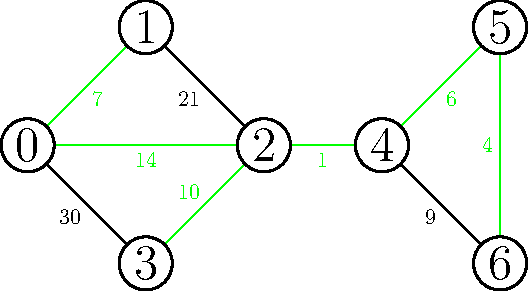
\includegraphics[scale = 0.8]{asy_mst/mst.pdf}
\end{figure}

Gli archi in verde costituiscono la soluzione ottima (in questo caso l'albero ricoprente di peso minimo è unico).

\end{document}
